\section{Projekt Bazy Danych}
    \subsection{Relacyjna baza dnaych SQL}
        Struktura oparta jest na modelu relacyjnym. Serwer SQL jest platformą, która obsługuje taką bazę danych, umożliwiając przechowywanie, zarządzanie oraz wykonywanie zapytań do tych danych.\\

        Modele relacyjne baz danych korzystają z relacji między tabelami, wykorzystując klucze główne i obce do ustanawiania powiązań. Dzięki językowi zapytań SQL (Structured Query Language) serwer SQL może zarządzać danymi, umożliwiając operacje takie jak wstawianie, odczyt, aktualizację i usuwanie informacji z tych tabel.\\
        
        Serwer SQL zapewnia efektywne zarządzanie bazą danych, a także zabezpieczenia, optymalizację oraz skalowalność. To narzędzie umożliwia obsługę wielu użytkowników jednocześnie, kontrolę nad dostępem do danych oraz wykonywanie złożonych operacji na danych przechowywanych w bazie relacyjne

    \subsection{Model bazy danych - Opis}
        \lstinputlisting[language=SQL]{./src/code_snippets/oop-php/src/sql/baza.sql}  

            Kod SQL definiuje strukturę bazy danych dla systemu zarządzania informacjami o piłkarzach.

            \begin{enumerate}
                \item Tworzenie bazy danych:\\
                Kod rozpoczyna od próby usunięcia bazy danych \textbf{pilkanozna} (jeśli istnieje) i następnie tworzy nową bazę o tej samej nazwie.
                Następnie wybiera tę nowo utworzoną bazę jako aktywną dla dalszych operacji.
                \item  Definicje tabel:
                \begin{itemize}
                    \item Tabela \textbf{pilkarz} przechowuje informacje o piłkarzach, takie jak imię, nazwisko, dane osobowe, umiejętności piłkarskie i pochodzenie.
                    \item Tabela \textbf{awatar} zawiera linki do obrazów reprezentujących piłkarzy.
                    \item Tabela \textbf{krajpilkarza} przechowuje informacje o krajach, do których należą piłkarze.
                    \item Tabela \textbf{numernakoszulce} zawiera numery na koszulkach piłkarzy.
                    \item Tabela \textbf{pozycja} zawiera różne pozycje, na których piłkarze mogą grać.
                \end{itemize}
                             
                \item Wstawianie danych:\\
                Dodaje przykładowe dane do tabeli \textbf{pozycja}, \textbf{numernakoszulce} i \textbf{krajpilkarza}.
            \end{enumerate}

        \subsubsection{Ustawienie uprawnień dla użytkownika}
        \begin{lstlisting}
CREATE USER "projekt"@"localhost" IDENTIFIED BY "Pracownia107!"; 
GRANT ALL PRIVILEGES ON pilkanozna.* TO "projekt"@"localhost";
        \end{lstlisting}

    \pagebreak
    \subsection{Rysunek}
        \begin{figure}[!htb]
            \centering
            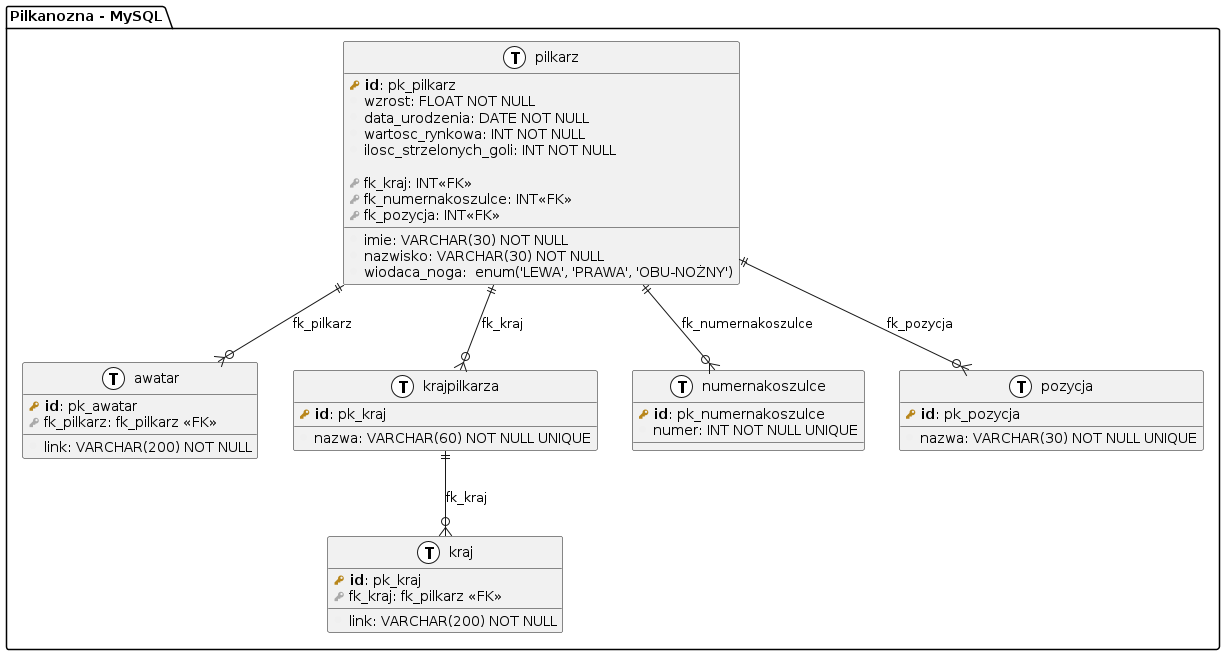
\includegraphics[width=0.9\textwidth]{diagramy/bazy.png}
            \caption{Diagram tabel bazy danych pilkanozna}
        \end{figure}